\section{Star-Matching}

\subsection{Introduction}

The goal of Star-Matching is to match the stars identified in an image to its corresponding star from the Star-Catalogue. This process of \textit{"tagging"} an image star with the Star-ID of its catalogue counterpart is the most complicated task for
any algorithm, and different algorithms can be distinguished mainly by how well they accomplish this task. 
If no match is found for an image star, it is tagged as a false star. Certain Star-Matching algorithms also provide for a verification step, which can rule out false matches that might have occurred at the end of the Star-Matching process.

Generally the matching is done by comparing the Star-Catalogue information to stars detected in the image. Despite the fact that catalogues also include brightness intensity as well as location information of stars, brightness is rarely used as filter in the process of Star-Matching. It has been shown that the probability of correct star matches is significantly influenced by the errors in estimation of star brightness, when brightness-based algorithms are used \cite{accardo2002brightness}.
Since the catalogues store visual magnitude of stars, whereas the brightness of the stars on an image is sensitive to the instruments, the process of predicting the image star's brightness from the catalogue star's brightness value is not a trivial process. In addition to this, brightness values are also considerably affected by noise and sensor malfunctions.

A Star-Matching algorithm, needs to match a minimum of two stars from an image to its respective catalogue star in order for the estimation algorithm to estimate the attitude. 
Matching more image stars, leads to an increased accuracy in the attitude estimate. Hence, for a given Star Tracker, a certain number of stars have to be matched in every image in order for the attitude to be accurate. This number is a fixed threshold ($N_{TH}$) for the system.

Star-Matching algorithms are of two distinct types, which arises from the two distinct modes in which a Star Tracker operates.
When it is first activated, a Star Tracker has no information about the satellite’s orientation (\textit{attitude}). This is known as the \textbf{Lost-in-Space (LIS) mode}. However, once the initial attitude has been found, it enters into the \textbf{Tracking mode}, which aids the algorithm in
estimating the attitude in the subsequent images. This involves predicting the current attitude accurately from
previously obtained information (the previous attitude and the angular velocity rates).


\subsection{Lost-in-Space}
\subsubsection{Introduction}

As mentioned earlier, a Star Tracker operates in the Lost-in-Space mode when it has no \textit{a priori} information of the attitude. Such cases occur when the STADS module is turned on for the first time, or when the Tracking mode fails.

A literature survey was performed to select a suitable algorithm for the Lost-in-Space mode. A few algorithms stood out in particular over the course of the survey. These algorithms, or a variant of the said, appeared to be used commonly, either due to their relatively simple implementation, their efficient and shorter run-time process, and their robustness to noise and false star-like objects that could enter the FOV.
Some of these algorithms are mentioned in detail.

\subsubsection{Planar Triangle Star Identification Technique}

This algorithm \cite{mcbryde2012star} analyzes the triangles formed by three stars at a time, matching the patterns using characteristics of the triangle. These characteristics include the area and polar moment of the triangle calculated using Herons’s formula. 
Then using a search method such as the \textbf{k-vector} (\textit{a search-less method}) \cite{mortari2014k}, all the triangles whose characteristics lie within one standard deviation of the observed triangle's are found. 
If more than one catalogue triangle meets the area and polar moment criteria, another star from the image is selected to identify and see how many stars overlap the two lists. If only two stars overlap then the triangle is identified. Else the solution is discarded and the algorithm works on a new star triangle formed by the image stars. 
Once three stars have been identified, the remaining stars in the image can be identified using a pivoting process. 

In their testing of the algorithm, out of 200 runs, it returned a false positive twice. This algorithm was implemented on hardware as well. 
However, this was one of the earliest Star-Matching methods that was developed. More robust and faster implementations have since been developed, and thus this algorithms was not considered.

\subsubsection{Shortest Distance Transform Technique}

This algorithm \cite{delabie2013highly} generates images using the star catalogue with a window that is slightly bigger than the FOV. These images are generated in such a way so as to cover the entire celestial sphere - Fig \ref{fig:sphere}. 
The generation of images requires one to distribute points on a sphere that is equidistant, and separated by the FOV angles.

\begin{figure}[h]
    \centering
    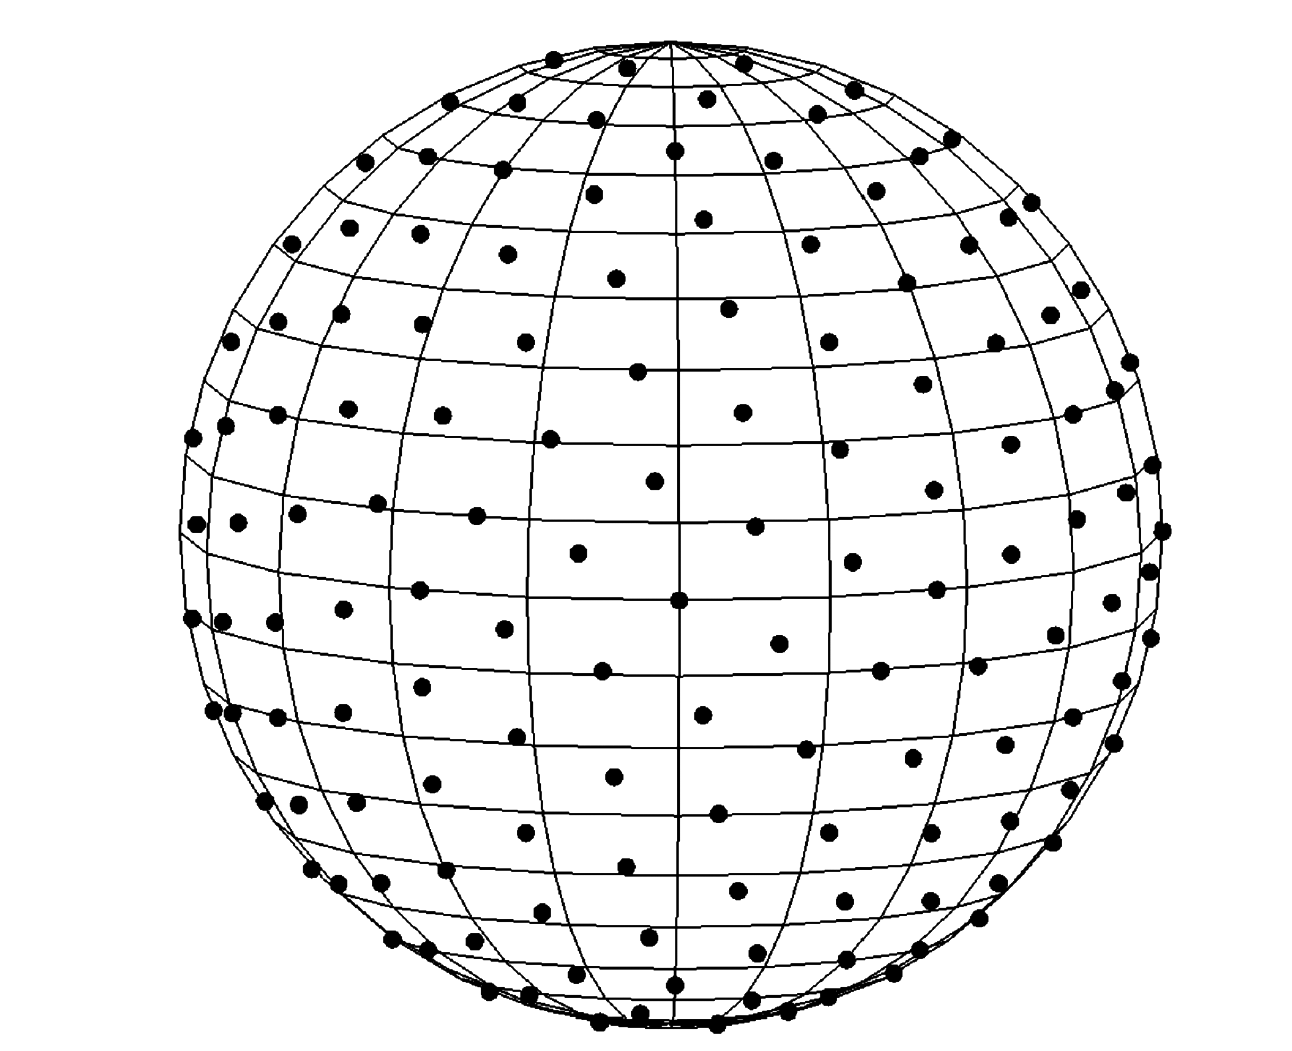
\includegraphics[scale = 0.25]{Figures/GNC/shortest_dist_sphere.png}
    \caption{Equidistant points on a sphere}
    \label{fig:sphere}
\end{figure}
Once these images are generated for the entire celestial sphere, the image from the sensor is taken.

The image from the sensor is compared with respect to all of the generated images. Two methods can be employed to compare the images:

\begin{itemize}
    \item \textbf{Two-Brightest-Stars Method}
    
    \begin{figure}[h!]
        \centering
        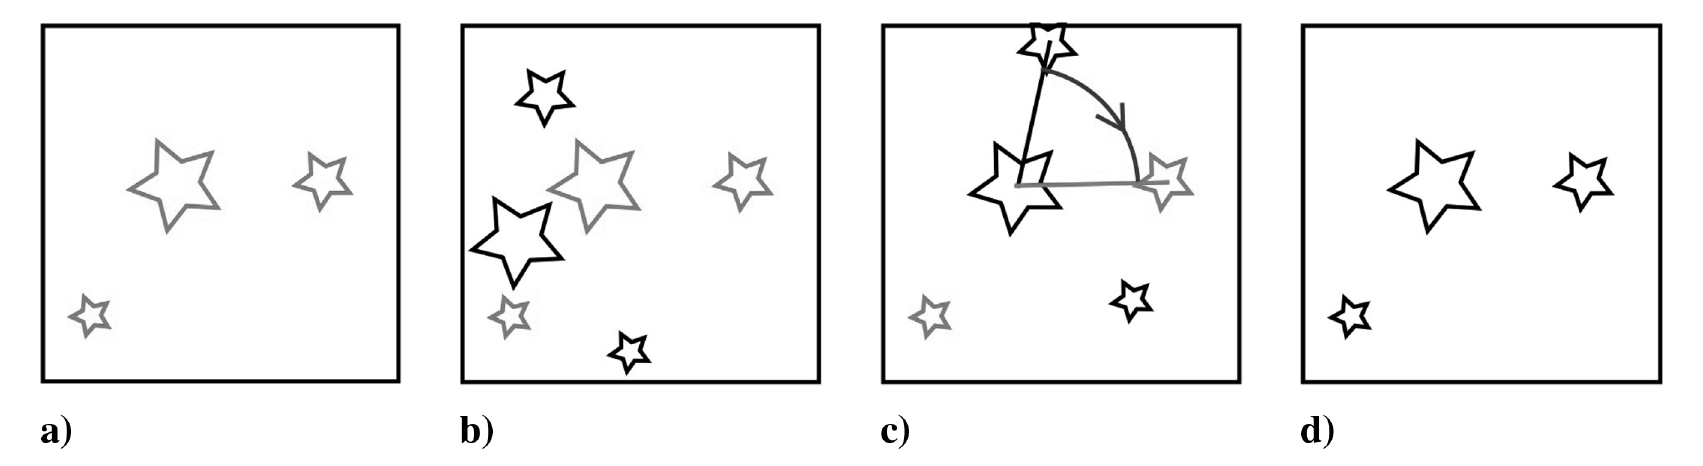
\includegraphics[scale=0.35]{Figures/GNC/shortest_dist_2_brightest.PNG}
        \caption{Shortest Distance Transform Technique: Two-brightest-stars Method}
    \end{figure}
    
    The brightest star from the generated image is placed in the same position as the brightest star from the captured image, thereby solving the translation problem. 
    Following which, the second brightest star from the captured image is rotated toward the second brightest star of the generated image. This is called the rotation step which ends up matching the images.
    
    \item \textbf{Centroid Method}
    
    \begin{figure}[h!]
        \centering
        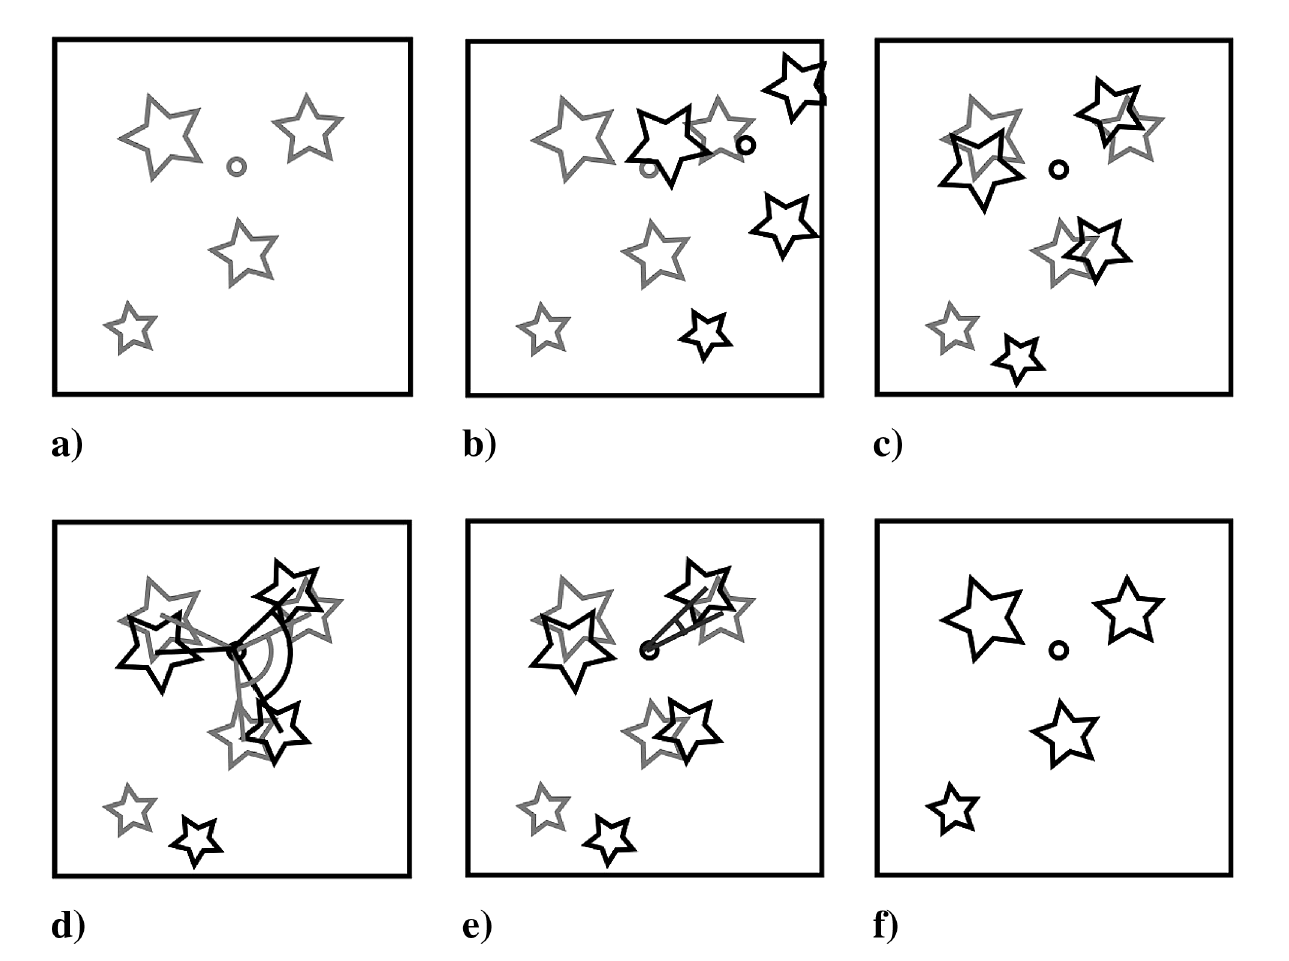
\includegraphics[scale=0.35]{Figures/GNC/shortest_dist_centroid.PNG}
        \caption{Shortest Distance Transform Technique: Centroid Method}
    \end{figure}
    
    This method uses the individual centroids of the $N$ brightest stars as well as the center of these centroids, obtained from the captured image to solve for the translation problem. 
    Vectors between the center to the individual centroids of the stars are calculated. These vectors are then rotated, so that they vectors from the captured image aligns with that of the vectors from the generated image. This procedure results in the matching of the centre and roll angle of the images.
\end{itemize}

In their testing, the computational time of the algorithm with the centroid method was one-third lower when the six brightest stars were used. The execution time of the algorithm was said to increase linearly with the number of pixels.
An important point to be noted here is that the algorithm is capable of accurately determining whether the offered solution is the correct one.
This algorithm could support both the LIS and Tracking mode, besides having been extensively tested with a variety of distortions in the captured image.

This algorithm was initially considered, when we intended on using the \textit{Attitude estimation using image matching technique} (refer \ref{sec:AIM}), which required a corresponding star-matching  algorithm that worked directly on the image coordinates and not the unit-vectors for faster computational performance. 

However, when QUEST was finalized as the estimation algorithm for the system, which implied the constraints of AIM no longer applied. Thus it was decided to proceed with a Star-Matching algorithm that had been tested and implemented on actual hardware, or actual space-based missions.


\subsubsection{Radial and Cyclic Star Matching Technique}

This algorithm \cite{zhang2008full} requires the centroids to be in polar coordinates $(r, \theta)$ instead of Cartesian $(x, y)$ coordinates.

\begin{itemize}
    \item \textbf{Radial Matching}
    
    \begin{figure}[!h]
        \centering
        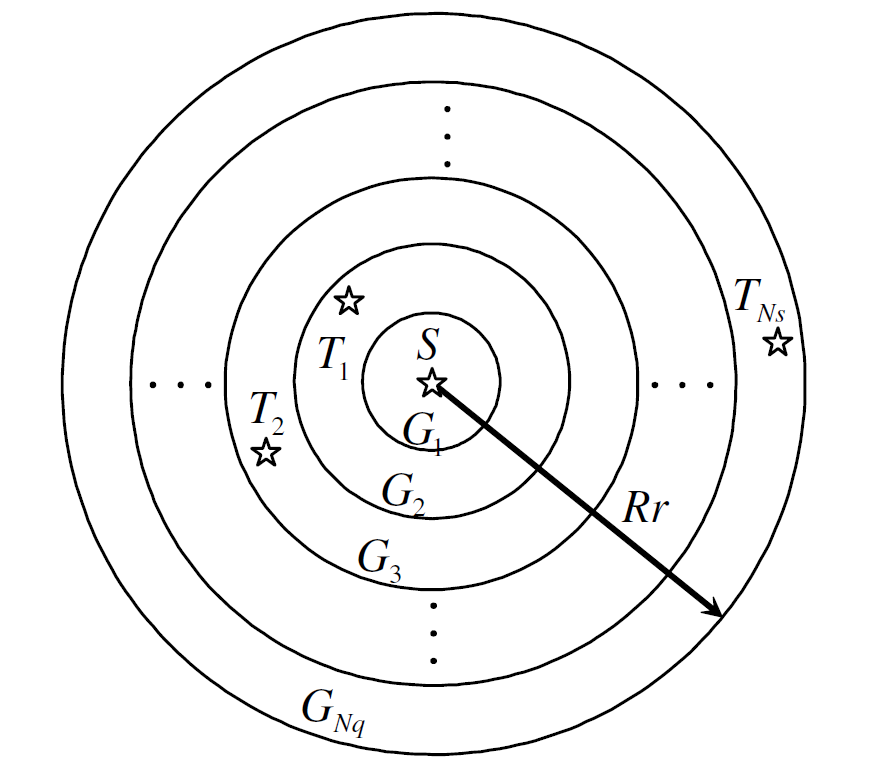
\includegraphics[scale=0.35]{Figures/GNC/radial_technique.PNG}
        \caption{Radial Matching Technique}
        \label{fig:radial}
    \end{figure}
    
    A reference star $S$, is chosen and all the other stars in the image are called neighbour stars - $(T_i)$ of $S$, by considering the reference star $S$ as the centre. Following which the area surrounding $S$ is divided into $N_q$ uniformly spaced strips, where each strip represents an angular distance of $R_r/N_q$. $R_r$ here is the maximum radial pattern radius. 
    
    An array of size $N_q$ is generated with all the elements initialized to $0$. If a star exists in the $i^{th}$ strip, then the $i^{th}$ element of the array becomes $1$. Thus this array represents the radial pattern of the reference star - $S$ - $pat_r (S)$.
    
    \item \textbf{Cyclic Matching}
    
    \begin{figure}[!h]
        \centering
        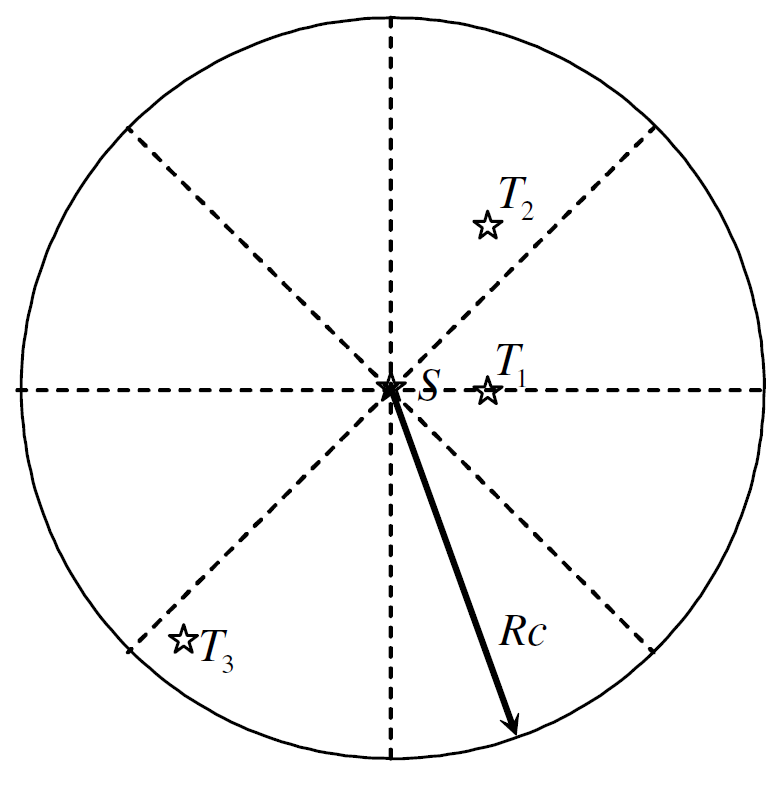
\includegraphics[scale=0.35]{Figures/GNC/cyclic_technique.PNG}
        \caption{Cyclic Matching Technique}
        \label{fig:cyclic}
    \end{figure}
    
    Using a similar reference star and neighbouring star technique, with the reference star $S$ being set as the centre and a suitable cyclic pattern radius of $R_c$, the central angles between neighbour stars are calculated, i.e, $\angle T_i S T_j$ ,$\forall$ $i\neq j$. The smallest angle $\angle T_l S T_k$ is selected and the side $ST_l$ is made the starting side. The image is then evenly partitioned into $8$ sectors. 
    
    An array of length $8$, similar to the radial pattern of $S$ is generated. If a star is found in the $i^{th}$ sector, then the $i^{th}$ place of the array becomes $1$.

\end{itemize}

The radial pattern and cyclic pattern arrays are used as a reference and searched upon in the processed catalogue to find stars that have similar pattern arrays. Thus it is required to have generated such pattern arrays for all the stars of the catalogue. This data is stored in the form of a lookup table for faster access.

In its testing through simulations, the star identification rate increases with increasing $R_r$, and an appropriate $N_q$ needs to be selected.

This method was considered as, since the FPGA-based implementation of this algorithm \cite{zhao2017real}, claimed to be faster than traditional implementations of Star-Matching algorithms on a micro-controller.